\section{Euclidean Spaces and Lattices}

\begin{enumerate}
	\item Let
	\[
	\mathbf{x}=(1,-2,3), \qquad \mathbf{y}=(4,0,-1).
	\]
	Compute \(\langle \mathbf{x},\mathbf{y}\rangle\), \(\|\mathbf{x}\|\), \(\|\mathbf{y}\|\), and \(\|\mathbf{x}+\mathbf{y}\|\).
	\item Determine whether the following sets are lattices in \(\mathbb{R}^2\):
	\begin{enumerate}
		\item $\mathbb{Z}^2$
		\item $\{(a,\sqrt{2}a): a\in\mathbb{Z}\}$
		\item $\{a(1,0)+b(1/2,1): a,b\in\mathbb{Z}\}$
		\item $\mathbb{Q}^2$
	\end{enumerate}
	\item Let
	\[
	\mathbf{b}_1=
	\begin{pmatrix}
		2\\0
	\end{pmatrix},
	\qquad
	\mathbf{b}_2=
	\begin{pmatrix}
		1\\1
	\end{pmatrix}.
	\]
	Describe explicitly the real span of \(\mathbf{b}_1,\mathbf{b}_2\), and the lattice generated by them.

	\item Show that if \(\mathbf{b}_1,\dots,\mathbf{b}_m\in \mathbb{R}^n\) are linearly independent, then
	\[
	\Lambda=\left\{\sum_{i=1}^m z_i\mathbf{b}_i : z_i\in\mathbb{Z}\right\}
	\]
	is a discrete subgroup of \(\mathbb{R}^n\).
	
	\item Give two distinct bases of the same lattice in \(\mathbb{R}^2\).

	\item Let \(B=[\mathbf{b}_1\ \mathbf{b}_2]\) with
	\[
	\mathbf{b}_1=
	\begin{pmatrix}
		1\\2
	\end{pmatrix},
	\qquad
	\mathbf{b}_2=
	\begin{pmatrix}
		3\\4
	\end{pmatrix}.
	\]
	Write \(\mathcal L(B)\) explicitly.
	
	\item Show that a lattice may have infinitely many bases.

	\item Let \(\Lambda\subseteq \mathbb{R}^n\) be a lattice. Prove that \(\Lambda\) is countable.
	\item Show that every lattice contains the zero vector and is closed under addition and negation.
	\item Let
	\[
	\Lambda=\{(2a+b,b): a,b\in\mathbb{Z}\}.
	\]
	Find a basis matrix \(B\) such that \(\Lambda=\mathcal L(B)\).
\end{enumerate}

\section{Gram--Schmidt Orthogonalization}

%\begin{enumerate}
%	\setcounter{enumi}{10}
%	\item Apply the Gram--Schmidt process to
%	\[
%	\mathbf{b}_1=
%	\begin{pmatrix}
%		1\\1
%	\end{pmatrix},
%	\qquad
%	\mathbf{b}_2=
%	\begin{pmatrix}
%		1\\0
%	\end{pmatrix}.
%	\]
%	
%	\item Apply the Gram--Schmidt process to
%	\[
%	\mathbf{b}_1=
%	\begin{pmatrix}
%		1\\0\\0
%	\end{pmatrix},
%	\quad
%	\mathbf{b}_2=
%	\begin{pmatrix}
%		1\\1\\0
%	\end{pmatrix},
%	\quad
%	\mathbf{b}_3=
%	\begin{pmatrix}
%		1\\1\\1
%	\end{pmatrix}.
%	\]
%	
%	\item Let \(\mathbf{b}_1,\mathbf{b}_2\in \mathbb{R}^n\) be linearly independent. Show that
%	\[
%	\mathbf{b}_2^*=\mathbf{b}_2-\frac{\langle \mathbf{b}_2,\mathbf{b}_1\rangle}{\langle \mathbf{b}_1,\mathbf{b}_1\rangle}\mathbf{b}_1.
%	\]
%	
%	\item Prove that the Gram--Schmidt vectors \(\mathbf{b}_1^*,\dots,\mathbf{b}_m^*\) are pairwise orthogonal.
%	
%	\item Prove that
%	\[
%	\mathrm{span}_{\mathbb{R}}(\mathbf{b}_1,\dots,\mathbf{b}_m)
%	=
%	\mathrm{span}_{\mathbb{R}}(\mathbf{b}_1^*,\dots,\mathbf{b}_m^*).
%	\]
%	
%	\item Show by example that Gram--Schmidt does not in general preserve the lattice generated by the basis vectors.
%	
%	\item Let
%	\[
%	\mathbf{b}_1=
%	\begin{pmatrix}
%		2\\0
%	\end{pmatrix},
%	\qquad
%	\mathbf{b}_2=
%	\begin{pmatrix}
%		3\\1
%	\end{pmatrix}.
%	\]
%	Compute \(\mu_{2,1}\) and \(\mathbf{b}_2^*\).
%	
%	\item Show that if the basis \(\mathbf{b}_1,\dots,\mathbf{b}_n\) is orthogonal, then \(\mathbf{b}_i^*=\mathbf{b}_i\) for all \(i\).
%	
%	\item Let \(\mathbf{b}_1,\dots,\mathbf{b}_n\) be linearly independent. Show that
%	\[
%	\mathbf{b}_i=\mathbf{b}_i^*+\sum_{j=1}^{i-1}\mu_{i,j}\mathbf{b}_j^*.
%	\]
%	
%	\item Explain why Gram--Schmidt is a geometric tool rather than a lattice basis reduction algorithm.
%\end{enumerate}

\newpage
\section{Fundamental Parallelepipeds and Determinants}
\begin{tcolorbox}
Let \( B: \mathbb{R}^n \to \mathbb{R}^n \) be an invertible linear map. Define the lattice \( \Lambda \) and the fundamental parallelepiped \( \mathcal{P}(B) \) by
\[
\Lambda = \mathcal{L}(B) = \{B\mathbf{z} : \mathbf{z} \in \mathbb{Z}^n\}\quad\text{and}\quad
\mathcal{P}(B) = \{B\boldsymbol{\alpha} : \boldsymbol{\alpha} \in [0,1)^n\}.
\]
Then \( \mathbb{R}^n \) admits the following disjoint decomposition:
\[
\mathbb{R}^n = \bigcup_{\boldsymbol{\lambda} \in \Lambda} \bigl({\lambda} + \mathcal{P}(B)\bigr),
\]
where for any \( \boldsymbol{\lambda}_1, \boldsymbol{\lambda}_2 \in \Lambda \),
\[
\bigl(\boldsymbol{\lambda}_1 + \mathcal{P}(B)\bigr) \cap \bigl(\boldsymbol{\lambda}_2 + \mathcal{P}(B)\bigr) = \varnothing \quad \text{whenever} \quad \boldsymbol{\lambda}_1 \neq \boldsymbol{\lambda}_2.
\]
\end{tcolorbox}
\begin{center}
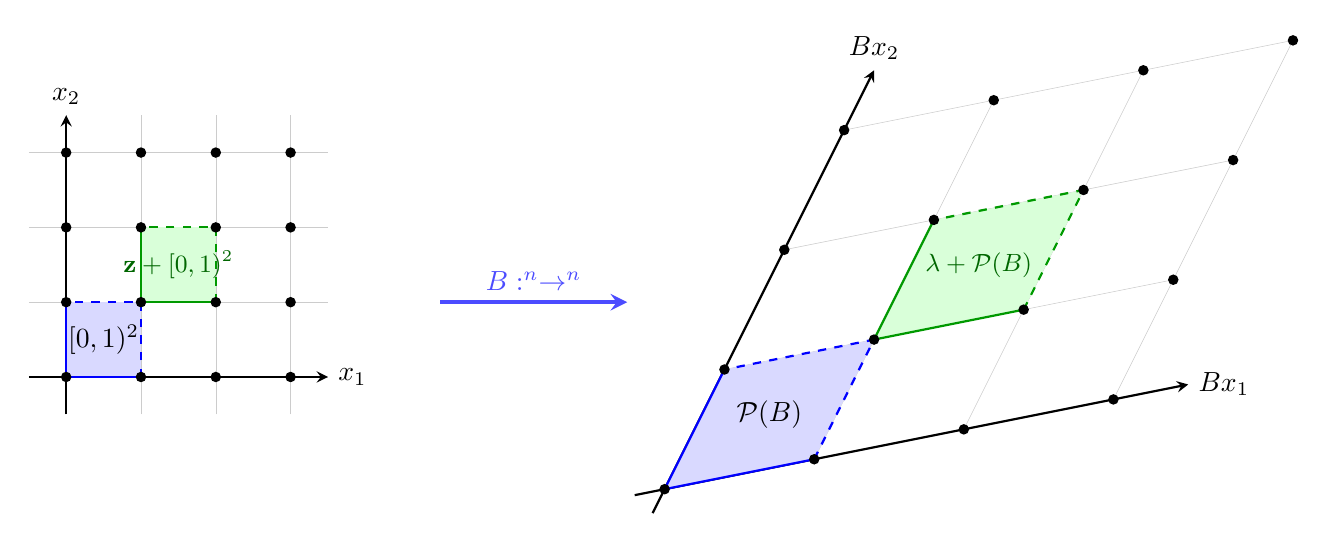
\begin{tikzpicture}[>=stealth, scale=.95]
	% ==========================================
	% LEFT SIDE: Original Space R^2 (Standard Lattice)
	% ==========================================
	\begin{scope}[yshift=1.5cm]
		% Grid and Axes
		\draw[step=1cm, gray!40, very thin] (-0.5,-0.5) grid (3.5,3.5);
		\draw[->, thick] (-0.5,0) -- (3.5,0) node[right] {$x_1$};
		\draw[->, thick] (0,-0.5) -- (0,3.5) node[above] {$x_2$};
		
		% Fundamental Domain [0,1)^2 at origin
		\fill[blue!15] (0,0) rectangle (1,1);
		\draw[blue, thick] (0,1) -- (0,0) -- (1,0); % Included boundaries
		\draw[blue, thick, dashed] (1,0) -- (1,1) -- (0,1); % Excluded boundaries
		\node at (0.5, 0.5) {$[0,1)^2$};
		
		% Translated Domain z + [0,1)^2
		\fill[green!15] (1,1) rectangle (2,2);
		\draw[green!60!black, thick] (1,2) -- (1,1) -- (2,1); % Included boundaries
		\draw[green!60!black, thick, dashed] (2,1) -- (2,2) -- (1,2); % Excluded boundaries
		\node[text=green!40!black] at (1.5, 1.5) {\small $\mathbf{z} + [0,1)^2$};
		
		% Draw Z^2 Lattice Points
		\foreach \x in {0,1,2,3} {
			\foreach \y in {0,1,2,3} {
				\fill[black] (\x,\y) circle (2pt);
			}
		}
		
%		% Label for the left side
%		\node[below] at (1.5, -1) {\textbf{Standard Lattice} $\mathbb{Z}^2$};
	\end{scope}
	
	% ==========================================
	% MAPPING ARROW
	% ==========================================
	% Represents the linear map B
	\draw[->, ultra thick, blue!70] (5, 2.5) -- (7.5, 2.5) node[midway, above] {$B:\R^n\to\R^n$};
	
	% ==========================================
	% RIGHT SIDE: Transformed Space R^2 (General Lattice)
	% ==========================================
	% We apply a custom basis to simulate the linear transformation B.
	\begin{scope}[xshift=8cm, yshift=0cm, x={(2cm, 0.4cm)}, y={(0.8cm, 1.6cm)}]
		
		% Transformed Grid
		\foreach \i in {0,1,2,3} {
			\draw[gray!40, very thin] (\i,0) -- (\i,3);
			\draw[gray!40, very thin] (0,\i) -- (3,\i);
		}
		
		% Transformed Axes
		\draw[->, thick] (-0.2,0) -- (3.5,0) node[right] {$Bx_1$};
		\draw[->, thick] (0,-0.2) -- (0,3.5) node[above] {$Bx_2$};
		
		% Fundamental Parallelepiped P(B) at origin
		\fill[blue!15] (0,0) -- (1,0) -- (1,1) -- (0,1) -- cycle;
		\draw[blue, thick] (0,1) -- (0,0) -- (1,0); % Included boundaries
		\draw[blue, thick, dashed] (1,0) -- (1,1) -- (0,1); % Excluded boundaries
		\node at (0.5, 0.5) {$\mathcal{P}(B)$};
		
		% Translated Parallelepiped \lambda + P(B)
		\fill[green!15] (1,1) -- (2,1) -- (2,2) -- (1,2) -- cycle;
		\draw[green!60!black, thick] (1,2) -- (1,1) -- (2,1); % Included boundaries
		\draw[green!60!black, thick, dashed] (2,1) -- (2,2) -- (1,2); % Excluded boundaries
		\node[text=green!40!black] at (1.5, 1.5) {\small $\boldsymbol{\lambda} + \mathcal{P}(B)$};
		
		% Draw \Lambda Lattice Points
		\foreach \x in {0,1,2,3} {
			\foreach \y in {0,1,2,3} {
				\fill[black] (\x,\y) circle (2pt);
			}
		}
		
%		% Label for the right side
%		\node[below] at (1.5, -0.625) {\textbf{Transformed Lattice} $\Lambda = \mathcal{L}(B)$};
	\end{scope}
\end{tikzpicture}
\end{center}

%\begin{proof}
%	Recall the standard decomposition of \( \mathbb{R}^n \) by translations of the half-open unit cube:
%	\begin{equation} \label{eq:standard_union}
%		\mathbb{R}^n = \bigcup_{\mathbf{z} \in \mathbb{Z}^n} \bigl(\mathbf{z} + [0,1)^n\bigr),
%	\end{equation}
%	where the sets are pairwise disjoint; that is, for \( \mathbf{z}_1, \mathbf{z}_2 \in \mathbb{Z}^n \),
%	\begin{equation} \label{eq:standard_disjoint}
%		\bigl(\mathbf{z}_1 + [0,1)^n\bigr) \cap \bigl(\mathbf{z}_2 + [0,1)^n\bigr) = \varnothing \quad \text{if} \quad \mathbf{z}_1 \neq \mathbf{z}_2.
%	\end{equation}
%	
%	Since \( B \) is a linear map, it distributes over vector addition. Thus, the image of a translated cube is the translated image of the cube:
%	\[
%	B\bigl(\mathbf{z} + [0,1)^n\bigr) = B\mathbf{z} + B\bigl([0,1)^n\bigr) = \boldsymbol{\lambda} + \mathcal{P}(B),
%	\]
%	where \( \boldsymbol{\lambda} = B\mathbf{z} \in \Lambda \). 
%	
%	To prove that the translates of \( \mathcal{P}(B) \) cover \( \mathbb{R}^n \), we apply the map \( B \) to both sides of equation \eqref{eq:standard_union}. Because \( B \) is invertible, it is surjective, implying \( B(\mathbb{R}^n) = \mathbb{R}^n \). Furthermore, the image of a union of sets under a function is the union of their images. Therefore,
%	\[
%	\mathbb{R}^n = B(\mathbb{R}^n) = B\Biggl( \bigcup_{\mathbf{z} \in \mathbb{Z}^n} \bigl(\mathbf{z} + [0,1)^n\bigr) \Biggr) = \bigcup_{\mathbf{z} \in \mathbb{Z}^n} B\bigl(\mathbf{z} + [0,1)^n\bigr) = \bigcup_{\boldsymbol{\lambda} \in \Lambda} \bigl(\boldsymbol{\lambda} + \mathcal{P}(B)\bigr).
%	\]
%	This establishes the covering property.
%	
%	To prove pairwise disjointness, let \( \boldsymbol{\lambda}_1, \boldsymbol{\lambda}_2 \in \Lambda \) be distinct elements (\( \boldsymbol{\lambda}_1 \neq \boldsymbol{\lambda}_2 \)). By the definition of the lattice \( \Lambda \), there exist unique vectors \( \mathbf{z}_1, \mathbf{z}_2 \in \mathbb{Z}^n \) such that \( \boldsymbol{\lambda}_1 = B\mathbf{z}_1 \) and \( \boldsymbol{\lambda}_2 = B\mathbf{z}_2 \). Since \( B \) is an injective map, \( \boldsymbol{\lambda}_1 \neq \boldsymbol{\lambda}_2 \) necessitates that \( \mathbf{z}_1 \neq \mathbf{z}_2 \). 
%	
%	Because \( B \) is injective, it preserves the intersection of sets; that is, \( B(X \cap Y) = B(X) \cap B(Y) \). Applying \( B \) to both sides of equation \eqref{eq:standard_disjoint} yields
%	\begin{align*}
%		B\Bigl( \bigl(\mathbf{z}_1 + [0,1)^n\bigr) \cap \bigl(\mathbf{z}_2 + [0,1)^n\bigr) \Bigr) &= B(\varnothing) \\
%		B\bigl(\mathbf{z}_1 + [0,1)^n\bigr) \cap B\bigl(\mathbf{z}_2 + [0,1)^n\bigr) &= \varnothing \\
%		\bigl(\boldsymbol{\lambda}_1 + \mathcal{P}(B)\bigr) \cap \bigl(\boldsymbol{\lambda}_2 + \mathcal{P}(B)\bigr) &= \varnothing.
%	\end{align*}
%	Thus, the translates of the fundamental parallelepiped are mutually disjoint, completing the proof.
%\end{proof}

%	\item Let
%	\[
%	B=
%	\begin{pmatrix}
	%		2 & 1\\
	%		0 & 3
	%	\end{pmatrix}.
%	\]
%	Compute \(\det(B)\).
%	
%	\item Let
%	\[
%	B=
%	\begin{pmatrix}
	%		1 & 2\\
	%		2 & 5
	%	\end{pmatrix}.
%	\]
%	Compute \(\det(\mathcal L(B))\).
%	
%	\item Describe the fundamental parallelepiped associated with
%	\[
%	B=
%	\begin{pmatrix}
	%		1 & 1\\
	%		0 & 2
	%	\end{pmatrix}.
%	\]
%	
%	\item Show that if \(U\in \mathbb{Z}^{n\times n}\) is unimodular\footnote{A unimodular matrix is a square integer matrix having determinant $+1$ or $-1$.}, then
%	\[
%	\mathcal L(BU)=\Lambda(B).
%	\]
%	
%	\item Deduce that if \(U\) is unimodular, then
%	\[
%	\det(\mathcal L(BU))=\det(\mathcal L(B)).
%	\]
%	
%	\item Prove that for a full-rank matrix \(B\in \mathbb{R}^{n\times n}\),
%	\[
%	\det(\mathcal L(B))=|\det(B)|.
%	\]
%	
%	\item Compute
%	\[
%	\sqrt{\det(B^TB)}
%	\]
%	for
%	\[
%	B=
%	\begin{pmatrix}
	%		1 & 1\\
	%		0 & 2
	%	\end{pmatrix},
%	\]
%	and compare it with \(|\det(B)|\).
%	
%	\item Let
%	\[
%	B=
%	\begin{pmatrix}
	%		3 & 0\\
	%		0 & 2
	%	\end{pmatrix}.
%	\]
%	Compare the determinant of \(\Lambda(B)\) with that of \(\mathbb{Z}^2\).
%	
%	\item Show that the determinant of a lattice does not depend on the choice of basis.
%	
%	\item Let \(\mathbf{b}_1,\dots,\mathbf{b}_n\) be a basis of a full-rank lattice. Show that
%	\[
%	\det(\Lambda)=\prod_{i=1}^n \|\mathbf{b}_i^*\|.
%	\]

\begin{enumerate}
	\item[\textbf{21-24}] Let
	\[
	B=
	\begin{pmatrix}
		2&1\\
		0&3
	\end{pmatrix},
	\qquad
	\Lambda=\mathcal L(B),
	\qquad
	\mathcal P(B)=\{B\boldsymbol\alpha:\boldsymbol\alpha\in[0,1)^2\}.
	\]
\end{enumerate}

\begin{enumerate}
	\setcounter{enumi}{20}
	\item[]
	\item Compute \(B^{-1}\).
	\item[]\item For each of the following vectors \(\mathbf x\), compute
	\[
	\mathbf t=B^{-1}\mathbf x,
	\qquad
	\mathbf z=\lfloor \mathbf t\rfloor\in\mathbb Z^2,
	\qquad
	\boldsymbol\alpha=\mathbf t-\lfloor \mathbf t\rfloor\in[0,1)^2,
	\]
	and hence find the unique decomposition
	\[
	\mathbf x=B\mathbf z+B\boldsymbol\alpha.
	\]
	Use:
	\[
	\binom{7.4}{5.2},
	\qquad
	\binom{-1.3}{4.7},
	\qquad
	\binom{3}{-2.4},
	\qquad
	\binom{-5.8}{-0.2}\qquad\in\mathcal{L}(B).
	\]
	\item[]\item For each vector above, identify explicitly the lattice vector
	\[
	\mathbf y=B\mathbf z\in\mathcal L(B)
	\]
	and the point
	\[
	\mathbf p=B\boldsymbol\alpha\in\mathcal P(B)
	\]
	such that \(\mathbf x=\mathbf y+\mathbf p\).
	\item[]\item Check in each case that \(\mathbf p\in\mathcal P(B)\) by writing it in the form
	\[
	\mathbf p=\alpha_1\mathbf b_1+\alpha_2\mathbf b_2
	\qquad\text{with }0\le \alpha_1,\alpha_2<1.
	\]
\end{enumerate}

\vfill

\begin{enumerate}
	\item[\textbf{25-28}] Let
	\[
	B=
	\begin{pmatrix}
		1&2\\
		2&1
	\end{pmatrix},
	\qquad
	\Lambda=\mathcal L(B),
	\qquad
	\mathcal P(B)=\{B\boldsymbol\alpha:\boldsymbol\alpha\in[0,1)^2\}.
	\]
\end{enumerate}

\medskip

\begin{enumerate}
	\setcounter{enumi}{24}
	\item[]\item Compute the four vertices of \(\mathcal P(B)\).
	\item[]\item For each point \(\mathbf x\) below, determine the unique lattice vector \(\mathbf y\in\Lambda\) such that
	\[
	\mathbf x\in \mathbf y+\mathcal P(B).
	\]
	Also compute the corresponding \(\mathbf p\in\mathcal P(B)\) with
	\[
	\mathbf x=\mathbf y+\mathbf p.
	\]
	Use:
	\[
	\binom{4.2}{5.1},
	\qquad
	\binom{-0.7}{1.6},
	\qquad
	\binom{3.9}{-2.4},
	\qquad
	\binom{-3.3}{-4.8}\qquad\in\mathcal L(B).
	\]
	\item[]\item For each point, verify your answer by computing \(B^{-1}\mathbf x\) and separating its coordinates into integer parts and fractional parts.
	\item[]\item Pick one of the four points and draw the translate \(\mathbf y+\mathcal P(B)\) that contains it.
\end{enumerate}

\newpage
\begin{enumerate}
	\item[\textbf{29-33}] Let
	\[
	B=
	\begin{pmatrix}
		2&0&1\\
		1&1&0\\
		0&1&2
	\end{pmatrix},
	\qquad
	\Lambda=\mathcal L(B).
	\]
	For \(\mathbf x\in\mathbb R^3\), define its remainder modulo \(\Lambda\) by
	\[
	r_B(\mathbf x)=B\bigl(\{B^{-1}\mathbf x\}\bigr),
	\]
	where fractional parts are taken coordinatewise.
	
\end{enumerate}

\begin{enumerate}
	\setcounter{enumi}{28}
   \item[]\item Compute \(r_B(\mathbf x)\) for each of the following vectors:
\[
\mathbf x_1=
\begin{pmatrix}
	5.2\\
	3.7\\
	-1.4
\end{pmatrix},
\qquad
\mathbf x_2=
\begin{pmatrix}
	-0.6\\
	4.1\\
	2.3
\end{pmatrix},
\qquad
\mathbf x_3=
\begin{pmatrix}
	7.2\\
	5.7\\
	0.6
\end{pmatrix}.
\]
\item[]\item For each \(\mathbf x_i\), also compute the corresponding lattice vector
\[
\mathbf y_i=\mathbf x_i-r_B(\mathbf x_i)\in\Lambda.
\]
\item[]\item Decide which pairs among \(\mathbf x_1,\mathbf x_2,\mathbf x_3\) lie in the same coset modulo \(\Lambda\). Justify your answer by comparing their remainders.
\item[]\item For every pair that lies in the same coset, compute explicitly the lattice vector
\[
\mathbf x_i-\mathbf x_j\in\Lambda.
\]
\item[]\item Explain how these calculations illustrate the uniqueness of the representation
\[
\mathbf x=\mathbf y+\mathbf p,
\qquad
\mathbf y\in\Lambda,\ \mathbf p\in\mathcal P(B).
\]
\end{enumerate}

\newpage
\section{Successive Minima and Short Vector}

%\begin{enumerate}
%	\setcounter{enumi}{30}
%	\item For the lattice generated by
%	\[
%	\mathbf{b}_1=
%	\begin{pmatrix}
%		2\\0
%	\end{pmatrix},
%	\qquad
%	\mathbf{b}_2=
%	\begin{pmatrix}
%		0\\3
%	\end{pmatrix},
%	\]
%	determine \(\lambda_1(\Lambda)\).
%	
%	\item Determine \(\lambda_1(\mathbb{Z}^2)\) and \(\lambda_2(\mathbb{Z}^2)\).
%	
%	\item Let
%	\[
%	\mathbf{b}_1=
%	\begin{pmatrix}
%		1\\0
%	\end{pmatrix},
%	\qquad
%	\mathbf{b}_2=
%	\begin{pmatrix}
%		1\\2
%	\end{pmatrix}.
%	\]
%	Find several short nonzero vectors in \(\Lambda(\mathbf{b}_1,\mathbf{b}_2)\), and determine \(\lambda_1(\Lambda)\).
%	
%	\item Give an example of a lattice \(\Lambda\) with
%	\[
%	\lambda_1(\Lambda)=\lambda_2(\Lambda).
%	\]
%	
%	\item Prove that every lattice has a shortest nonzero vector.
%	
%	\item Explain why the determinant gives information about lattice density but not the exact value of \(\lambda_1(\Lambda)\).
%	
%	\item Let \(\Lambda=\mathbb{Z}^n\). Determine \(\lambda_i(\Lambda)\) for all \(1\le i\le n\).
%	
%	\item Show that if \(\Lambda'\subseteq \Lambda\), then
%	\[
%	\lambda_1(\Lambda)\le \lambda_1(\Lambda').
%	\]
%	
%	\item State a Minkowski-type upper bound for \(\lambda_1(\Lambda)\), and explain its meaning.
%	
%	\item Explain why Minkowski's theorem is existential rather than algorithmic.
%\end{enumerate}

%\section{SVP, CVP, and BDD}
%
%\begin{enumerate}
%	\setcounter{enumi}{40}
%	\item Let
%	\[
%	\Lambda=\mathbb{Z}^2,
%	\qquad
%	\mathbf{t}=
%	\begin{pmatrix}
%		0.3\\1.7
%	\end{pmatrix}.
%	\]
%	Find a closest lattice vector to \(\mathbf{t}\).
%	
%	\item Let
%	\[
%	\Lambda=\mathbb{Z}^2,
%	\qquad
%	\mathbf{t}=
%	\begin{pmatrix}
%		0.5\\0.5
%	\end{pmatrix}.
%	\]
%	Determine all closest lattice vectors to \(\mathbf{t}\).
%	
%	\item State precisely the difference between the Shortest Vector Problem and the Closest Vector Problem.
%	
%	\item State precisely the difference between the Closest Vector Problem and Bounded-Distance Decoding.
%	
%	\item Show that an exact algorithm for CVP yields an exact algorithm for BDD.
%	
%	\item Explain why the uniqueness promise in BDD makes it easier than general CVP.
%	
%	\item Let
%	\[
%	\Lambda=
%	\left\{
%	\begin{pmatrix}
%		2a\\2b
%	\end{pmatrix}
%	: a,b\in\mathbb{Z}
%	\right\},
%	\qquad
%	\mathbf{t}=
%	\begin{pmatrix}
%		1.2\\1.8
%	\end{pmatrix}.
%	\]
%	Find a closest lattice vector.
%	
%	\item Formulate the \(\gamma\)-approximate versions of SVP and CVP.
%	
%	\item Explain why approximation problems are often more relevant algorithmically than exact problems.
%	
%	\item Show that a solution to exact SVP also decides whether \(\lambda_1(\Lambda)\le r\), for any real \(r>0\).
%\end{enumerate}
%

\newpage
\section{Dual Lattices}
%
%\begin{enumerate}
%	\setcounter{enumi}{50}
%	\item Compute the dual lattice of \(\mathbb{Z}^n\).
%	
%	\item Let
%	\[
%	B=
%	\begin{pmatrix}
%		2 & 0\\
%		0 & 3
%	\end{pmatrix}.
%	\]
%	Compute a basis matrix for \(\Lambda(B)^*\).
%	
%	\item Verify directly that if \(B^*=(B^{-1})^T\), then
%	\[
%	\langle \mathbf{x},\mathbf{y}\rangle \in \mathbb{Z}
%	\]
%	for all \(\mathbf{x}\in \Lambda(B)\) and all \(\mathbf{y}\in \Lambda(B^*)\).
%	
%	\item Prove that
%	\[
%	\det(\Lambda^*)=\det(\Lambda)^{-1}
%	\]
%	for every full-rank lattice \(\Lambda\).
%	
%	\item Compute the dual lattice of the lattice generated by
%	\[
%	B=
%	\begin{pmatrix}
%		1 & 1\\
%		0 & 2
%	\end{pmatrix}.
%	\]
%	
%	\item Prove that \((\Lambda^*)^*=\Lambda\).
%	
%	\item Let \(\Lambda\subseteq \mathbb{R}^n\) be full rank. Show that \(\Lambda^*\) is a lattice.
%	
%	\item Explain the geometric meaning of the dual lattice.
%	
%	\item Show that if \(\Lambda_1\subseteq \Lambda_2\), then
%	\[
%	\Lambda_2^*\subseteq \Lambda_1^*.
%	\]
%	
%	\item Determine the dual of the lattice \(a\mathbb{Z}\subseteq \mathbb{R}\), where \(a>0\).
%\end{enumerate}
%
\section{Reduced Bases and the LLL algorithm}
%
%\begin{enumerate}
%	\setcounter{enumi}{60}
%	\item Explain the difference between a good basis and a bad basis of the same lattice.
%	
%	\item State the size-reduction condition in the definition of an LLL-reduced basis.
%	
%	\item State the Lov\'asz condition.
%	
%	\item Explain why LLL reduction uses the Gram--Schmidt data of a basis.
%	
%	\item Show that an orthogonal basis is automatically size-reduced.
%	
%	\item Explain why LLL does not generally solve exact SVP in high dimension.
%	
%	\item State the standard approximation guarantee for the first vector of an LLL-reduced basis.
%	
%	\item Explain why LLL is nevertheless useful in practice.
%	
%	\item Describe the qualitative shape of the Gram--Schmidt profile of a reduced basis.
%	
%	\item Give an example of a context in cryptography where one wants a public basis to be bad and a secret basis to be good.
%\end{enumerate}
%
\section{\(q\)-ary Lattices and SIS}
%
%\begin{enumerate}
%	\setcounter{enumi}{70}
%	\item Let \(q=5\) and
%	\[
%	A=
%	\begin{pmatrix}
%		1 & 2
%	\end{pmatrix}.
%	\]
%	Determine all \(\mathbf{z}=(z_1,z_2)^T\in \mathbb{Z}^2\) such that
%	\[
%	A\mathbf{z}\equiv 0 \pmod 5.
%	\]
%	
%	\item Let
%	\[
%	A\in \mathbb{Z}_q^{n\times m}.
%	\]
%	Show that
%	\[
%	\Lambda_q^\perp(A)=\{\mathbf{z}\in \mathbb{Z}^m : A\mathbf{z}\equiv \mathbf{0}\pmod q\}
%	\]
%	is a lattice.
%	
%	\item State the Short Integer Solution problem.
%	
%	\item Explain why SIS may be regarded as a shortest-vector-type problem in a \(q\)-ary lattice.
%	
%	\item Let
%	\[
%	A=
%	\begin{pmatrix}
%		1 & 1 & 1
%	\end{pmatrix}
%	\in \mathbb{Z}_3^{1\times 3}.
%	\]
%	Find a nonzero short vector in \(\Lambda_3^\perp(A)\).
%	
%	\item Explain why the requirement of shortness is essential in SIS.
%	
%	\item Compare the problems
%	\[
%	A\mathbf{z}\equiv 0 \pmod q
%	\qquad \text{and} \qquad
%	\text{SIS}(A,q,\beta).
%	\]
%	
%	\item Let \(q\mathbb{Z}^m\subseteq \Lambda\subseteq \mathbb{Z}^m\). Show that \(\Lambda\) is a \(q\)-ary lattice.
%	
%	\item Give an example of a large nonzero solution to a modular equation that would be useless in the context of SIS.
%	
%	\item Explain the relationship between modular linear relations and lattice geometry.
%\end{enumerate}
%
\section{Conceptual and Proof Exercises}
%
%\begin{enumerate}
%	\setcounter{enumi}{80}
%	\item Complete and explain the chain
%	\[
%	\text{linear algebra}
%	\longrightarrow
%	\text{Gram--Schmidt}
%	\longrightarrow
%	\text{lattices}
%	\longrightarrow
%	\text{basis reduction}
%	\longrightarrow
%	\text{hard problems}.
%	\]
%	
%	\item Prove that if \(U\in \mathbb{Z}^{n\times n}\) is unimodular, then \(U^{-1}\in \mathbb{Z}^{n\times n}\).
%	
%	\item Show that if \(B'\) and \(B\) are basis matrices of the same full-rank lattice, then
%	\[
%	B'=BU
%	\]
%	for some unimodular matrix \(U\).
%	
%	\item Prove that every exact algorithm for SVP yields an algorithm for the decision problem
%	\[
%	\text{``Is }\lambda_1(\Lambda)\le r\text{?''}
%	\]
%	
%	\item Prove that every exact algorithm for CVP yields an algorithm for BDD.
%	
%	\item Explain why exact lattice problems are usually harder than approximate lattice problems.
%	
%	\item Explain why bad bases hide geometric information.
%	
%	\item Explain how lattice reduction can reveal hidden small relations among integers.
%	
%	\item Explain why coefficient vectors of polynomials may be viewed as lattice vectors.
%	
%	\item Write a brief essay comparing the roles of SVP, CVP, and SIS in lattice-based cryptography.
%\end{enumerate}